
\begin{frame}{Defining the Probability Path}
    \begin{columns}
        \column{0.6\textwidth}
        \textbf{The Goal:} 
        We need to define a path for a particle to move from Noise ($x_0$) to Data ($x_1$).
        
        \vspace{0.5cm}
        
        \textbf{Optimal Transport}
        We choose the simplest geometric path: the \textbf{straight line}.
        
        \begin{block}{Interpolation Formula}
            $$ x_t = (1 - t)x_0 + t x_1 $$
        \end{block}
        
        \column{0.4\textwidth}
        \centering
        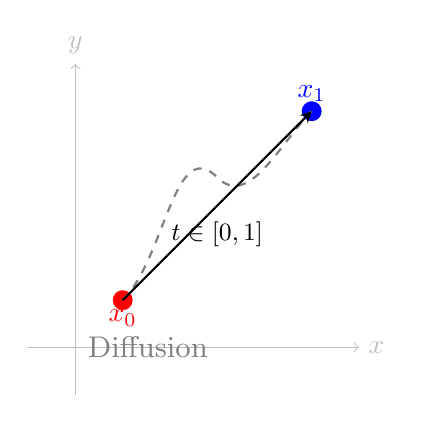
\begin{tikzpicture}[scale=1.2]
            % Axes
            \draw[->, lightgray] (-0.5,0) -- (3,0) node[right] {$x$};
            \draw[->, lightgray] (0,-0.5) -- (0,3) node[above] {$y$};
            
            % Points
            \fill[red] (0.5, 0.5) circle (3pt) node[below] {$x_0$};
            \fill[blue] (2.5, 2.5) circle (3pt) node[above] {$x_1$};
            
            % Diffusion models (dashed curve)
            \draw[dashed, gray, thick] (0.5, 0.5) to[out=45, in=135] (1.5, 1.8) to[out=315, in=225] (2.5, 2.5) node[midway, right] {\small Diffusion};
            
            % Flow matching (solid line)
            \draw[thick, ->, >=stealth] (0.5, 0.5) -- (2.5, 2.5) node[midway, above left] {};
            
            % Time label
            \node at (1.5, 1.2) {\small $t \in [0, 1]$};
        \end{tikzpicture}
        \end{columns}
\end{frame}

\begin{frame}{The Regression Target}
    The neural network needs to learn the \textbf{velocity field} $v_\theta(x, t)$ that generates this path.
    
    \vspace{0.5cm}
    
    Since the path is a straight line, the velocity is the time derivative:
    
    $$ u_t(x|x_1) = \frac{d}{dt} x_t = \frac{d}{dt} \left( (1 - t)x_0 + t x_1 \right) $$
    
    \vspace{0.5cm}
    
    \begin{alertblock}{The Key Advantage}
        The target velocity is \textbf{constant}:
        $$ u_t = x_1 - x_0 $$
    \end{alertblock}
    
    \vspace{0.3cm}
    $\Rightarrow$ The network learns a stable, constant direction for each pair, which is easier than learning a curved diffusion path.
\end{frame}

\begin{frame}{Sampling with Euler Method}
    \textbf{Inference:} Starting from noise $x_0$, we follow the learned velocity field.
    
    \begin{columns}
        \column{0.55\textwidth}

        We use the \textbf{Euler Integration}:
        $$ x_{t+dt} = x_t + v_\theta(x_t, t) \cdot dt $$
        
        \vspace{0.2cm}
        
        \textbf{Why it works well?}
        \begin{itemize}
            \item The learned trajectories are nearly straight (Optimal Transport).
            \item Low discretization error.
            \item Fast generation ($N=10$ to $20$ steps).
        \end{itemize}

        \column{0.4\textwidth}
        \begin{algorithm}
            \footnotesize
            \textbf{Algorithm: Sampling}
            \begin{enumerate}
                \item $x \leftarrow \text{SampleNoise}()$
                \item $dt \leftarrow 1/N$
                \item \textbf{For} $i = 0$ to $N-1$:
                \begin{itemize}
                    \item $v \leftarrow \text{Model}(x, t)$
                    \item $x \leftarrow x + v \cdot dt$
                    \item $t \leftarrow t + dt$
                \end{itemize}
                \item \textbf{Return} $x$
            \end{enumerate}
        \end{algorithm}
    \end{columns}
\end{frame}
